\section{XAI}
To address explainability, following the professors' advice, we decided to apply the methods discussed in class to better understand the decisions made by the best model (GBM with SMOTETomek) in classifying the data.
More specifically, we compared the native explanation of the \enquote{LGBMClassifier} with the \enquote{SHAP} explanation, using both interventional and distributional approaches on a subset of the dataset, as well as locally on individual instances. We also applied \enquote{LIME} and \enquote{LORE} for local explanations on individual instances, with the latter used to generate counterfactual rules.

\subsection{SHAP explanations}

We used the SHAP TreeExplainer to generate SHAP values for the Gradient Boosting Machine, testing it on the first 400 instances of the test set for computational efficiency. Two explanation approaches were applied: the interventional explanation algorithm which perturbs features based on a causal model, and the distributional explanation algorithm which conditions the distribution learned from the training data.

The SHAP beeswarm plot in \autoref{fig:beeswarm} highlights the primary factors influencing the model's predictions, with key features including \textit{avg\_relative\_position}, \textit{climb\_total}, and \textit{position\_entropy}. Average relative position consistently shows a strong positive impact, particularly for low values, while climb total exhibits a diverse and variable influence across the dataset, with lower values influencing positively. Top 20 entropy similarly to average relative position influences negatively for higher values and positively for lower ones. On the other hand, features like \textit{cyclist\_experience} and \textit{cyclist\_level} have minimal impact, as their SHAP values remain near zero. 
The plot suggests that the model's decisions align with expected trends: cyclists with lower average positions or lower entropy in their results are more likely to maintain a spot in the top 20.

From the distributional perspective, \textit{cyclist\_age} consistently has a negative effect, while \textit{climb\_total} and \textit{position\_entropy} exhibit greater variability, with lower values contributing to higher positive SHAP values. \textit{top\_20\_entropy} has a negative contribution for lower values and a positive contribution for higher values, which appears to contradict expectations. Finally, we observe that the features predominantly drive predictions toward negative outcomes, with only a few contributing modestly toward positive labels.

While the visualizations effectively highlight the critical features and their contributions, they also expose overlapping distributions and low-impact features, pointing to potential redundancy. 

\begin{figure}[H]
    \centering
    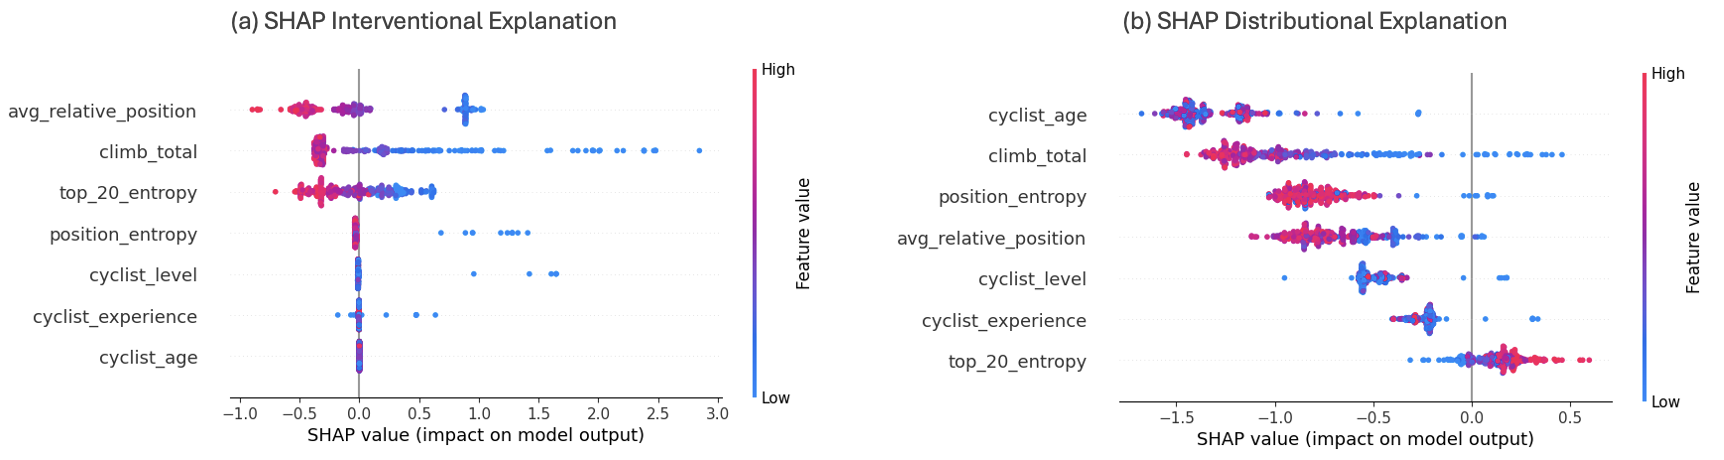
\includegraphics[width=0.9\linewidth]{images//XAI/beeswarm.png}
    \caption{\small SHAP beeswarm plot both for interventional and distributional approaches}
    \label{fig:beeswarm}
\end{figure}

\noindent In selecting features for the dependence plot, we prioritized the \textit{avg\_relative\_position} because it is one of the most important features for all methods. The feature found to be dependent is \textit{top\_20\_entropy}, another key feature. The plot in \autoref{fig:dependence_plot} shows the relationship between the two features in terms of SHAP values for the average relative position as the two vary.

The interventional explanation plot indicates that for \textit{average\_relative\_position} and \textit{top\_20\_entropy} values close to 0, the model predicts the highest SHAP value, suggesting a positive classification. This observation is reasonable, as low entropy and low average relative positions could indicate either a very strong cyclist or one with limited simpler race participation, where competing in simpler events often results in higher placements. As both entropy and average position increase, the SHAP value remains positive. This is because strong cyclists generally achieve good average placements but exhibit higher entropy due to strategic variations, as observed in \autoref{subsec:extra_analysis}. For intermediate values of the \textit{average\_relative\_position}, the SHAP value becomes insignificant both for higher or lower entropy.

For lower entropy values combined with higher average relative positions, the model tends to suggest a negative SHAP value. This is logical, as a cyclist with high average relative positions is unlikely to be very strong and its entropy is low because he typically places poorly.

\begin{figure}[H]
    \centering
    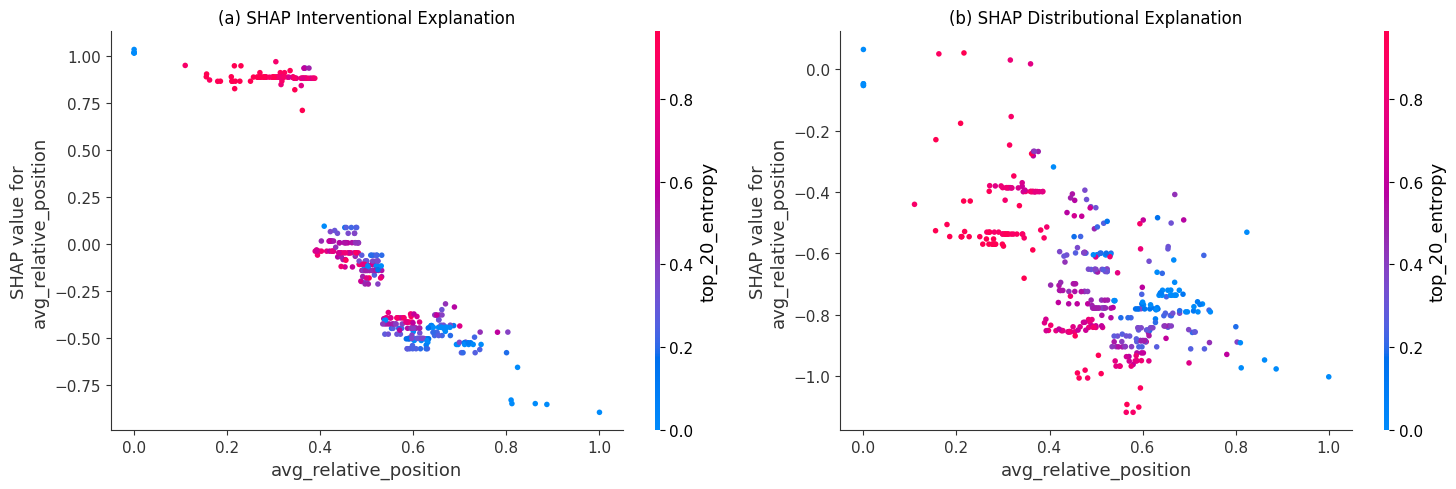
\includegraphics[width=0.9\linewidth]{images//XAI/dependence_plot.png}
    \caption{\small SHAP dependence plot both for interventional and distributional approaches}
    \label{fig:dependence_plot}
\end{figure}

The final SHAP analysis involves the difference in distributional and interventional approaches. The line plot in \autoref{fig:differences} (a) shows the distribution of maximum differences between interventional and distributional SHAP explanations for each instance. The peak around 1.4 indicates that most instances exhibit a maximum discrepancy of approximately 1.4, with a rapid drop in density beyond 1.6, suggesting large differences are rare. The narrow distribution indicates consistency, with only a few outliers showing significant differences. Overall, the two explanation methods generally agree, with limited divergence. 

The scatter plot in \autoref{fig:differences} (b) shows the maximum observed differences in SHAP values for each feature. Features like \textit{climb\_total} and \textit{cyclist\_age} exhibit the highest discrepancies, suggesting they may be more sensitive to the explanation method or involve complex interactions. In contrast, features such as \textit{top\_20\_entropy} and \textit{position\_entropy} show minimal differences, indicating stability across methods.

\begin{figure}[H]
    \centering
    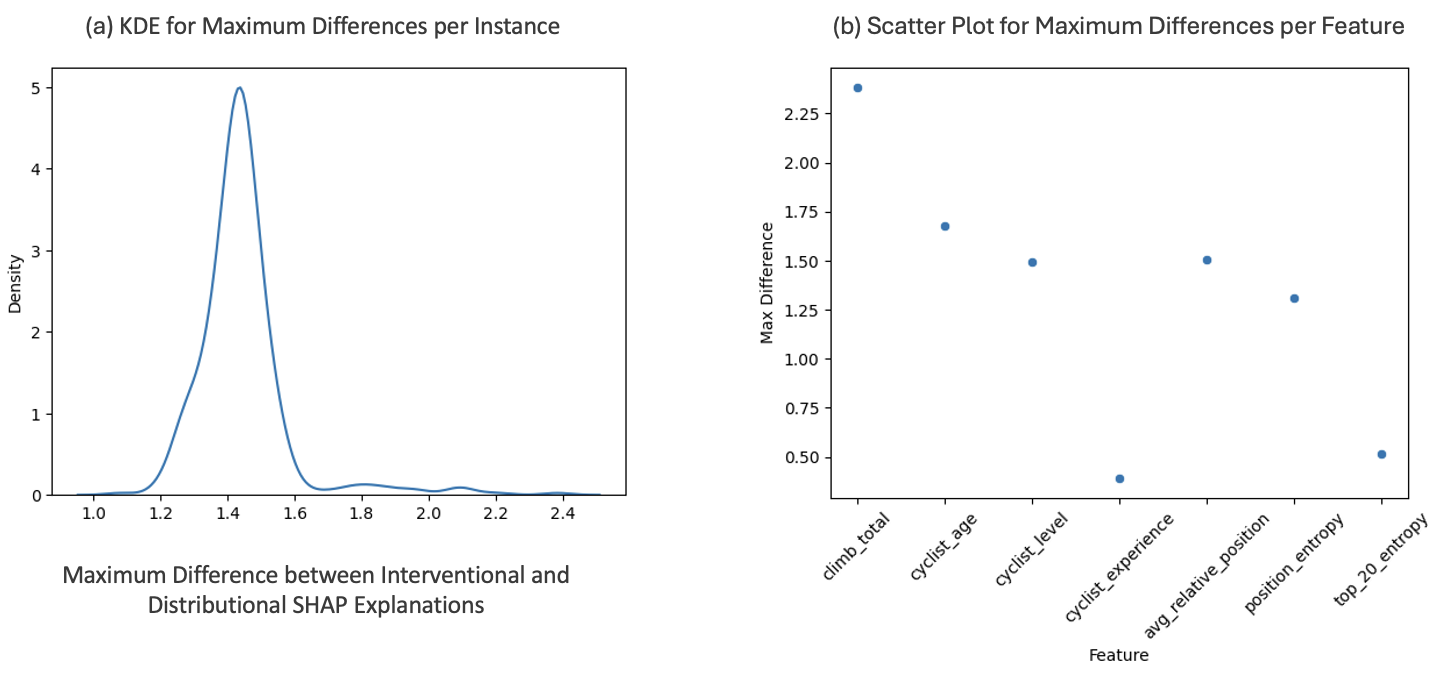
\includegraphics[width=0.8\linewidth]{images//XAI/differences.png}
    \vspace{-5pt}
    \caption{ \small SHAP explanation differences across instances (a) and features (b)}
    \label{fig:differences}
\end{figure}


\subsection{LORE local explanations and Counterfactual}
Regarding the LORE explanation, we focused on providing local explanations for individual data points, extracting rules, and counterfactuals, and assessing fidelity. Our focus is on understanding the conditions under which class 1 is predicted, given the models' low performance in this class.

In \autoref{fig:lore_tp} we observe the extracted rule (a) and most relevant counterfactuals (b) for random true positive data.
This rule indicates that the model heavily relies on the top 20 entropy and average relative position features. Specifically, the rule suggests that higher entropy combined with a lower average relative position is indicative of a strong cyclist. This may imply that cyclists with high entropy are highly experienced, while a low average relative position reflects consistently strong placements overall.
The high fidelity of 99.5\% reinforces the reliability of these observations.

\begin{figure}[H]
    \centering
    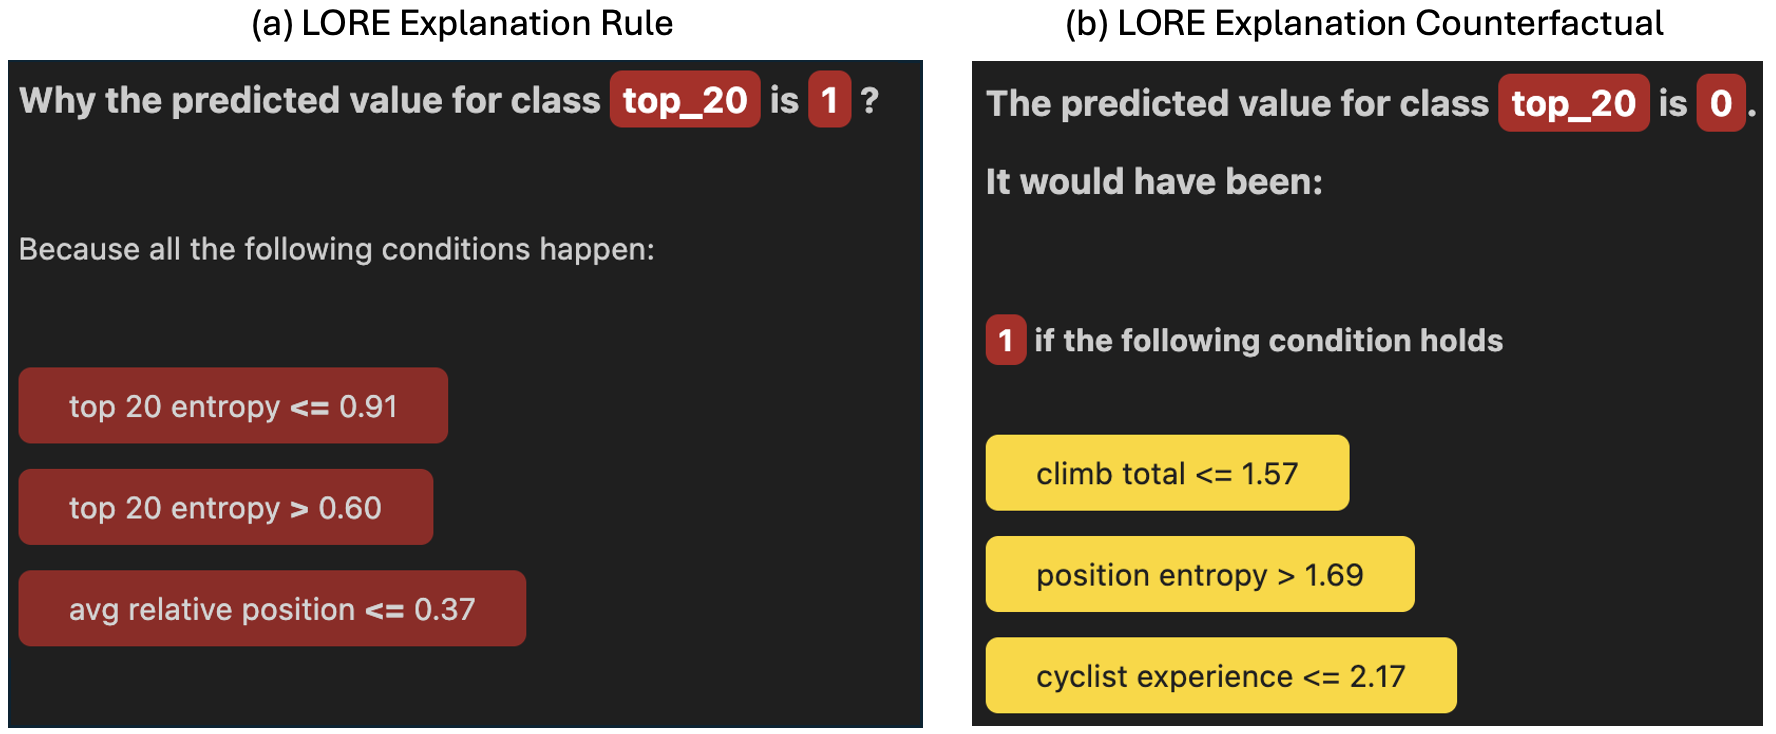
\includegraphics[width=0.7\linewidth]{images//XAI/lore_tp.png}
    \vspace{-5pt}
    \caption{ \small{LORE Rule (a) and Counterfactual (b) on True Positive Data}}
    \label{fig:lore_tp}
\end{figure}

\noindent \autoref{fig:lore_fn} shows the extracted rule (a) and most relevant counterfactuals (b) for a random false positive negative.

Low values of top 20 entropy and position entropy suggest the cyclist might be inexperienced, as consistent placements are unlikely to all be good. This may reflect a strategic focus on specific races or limited exposure to diverse scenarios, unlike experienced cyclists who show more varied results across conditions as seen also in the extra analysis. In fact, as counterfactuals, the model suggests a higher entropy and a low average relative position, indicating a good position until that race. The top 20 entropy value in this rule is not useful, as the maximum for this feature is 1.
Also in this case fidelity is very high (98.5\%), reinforcing the reliability of extracted rules.

\begin{figure}[H]
    \centering
    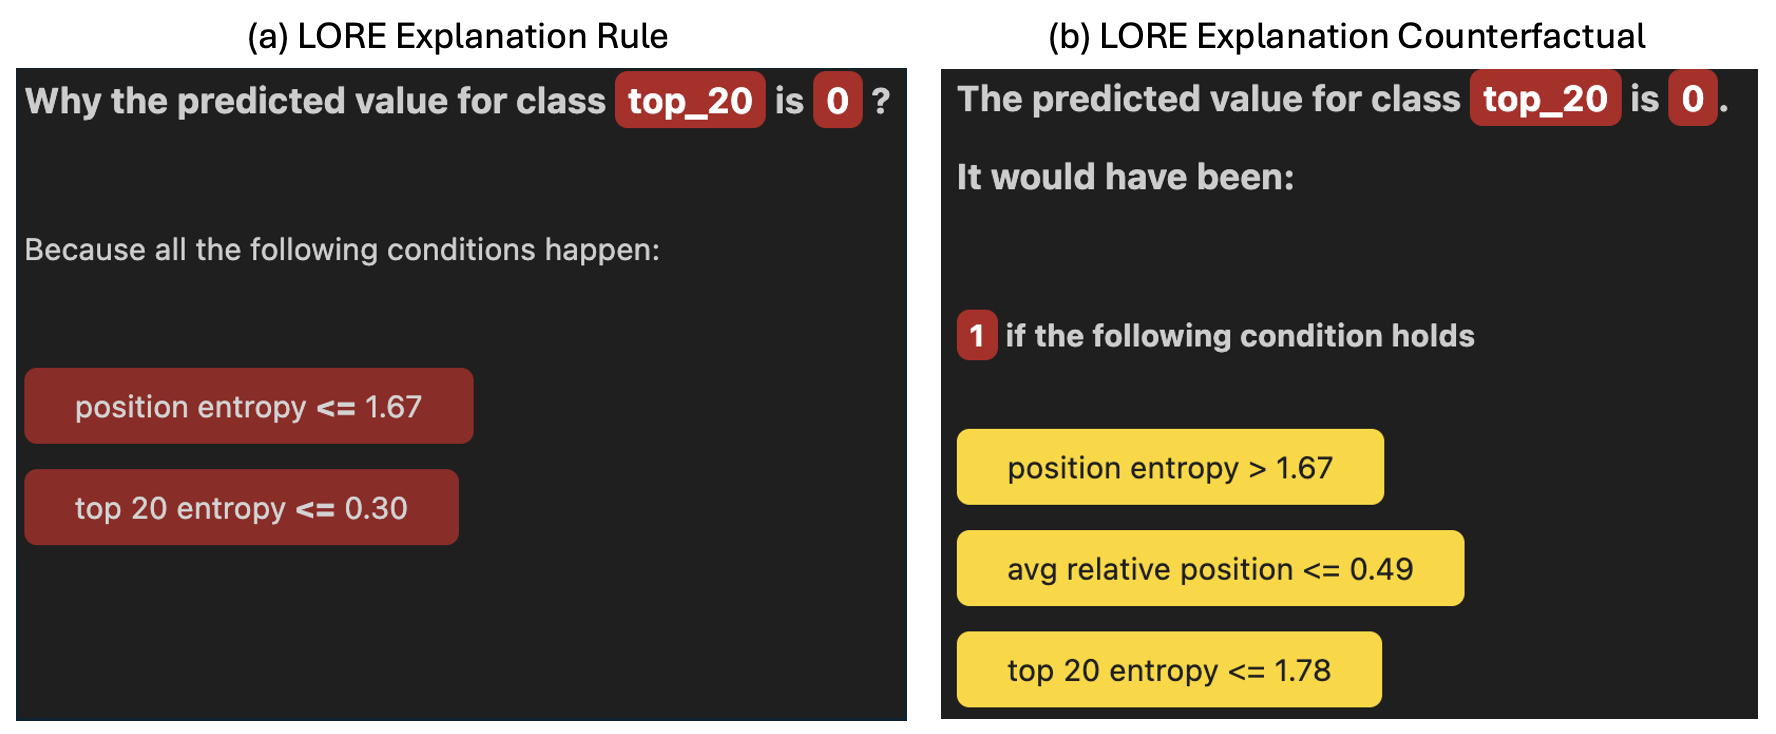
\includegraphics[width=0.7\linewidth]{images//XAI/lore_fn.png}
    \caption{ \small{LORE Rule (a) and Counterfactual (b) on False Negative Data}}
    \label{fig:lore_fn}
\end{figure}

\noindent Explanation rules and counterfactuals for true negative and false positive can be found in the notebook.

\subsection{LIME}

\noindent
\textbf{Analysis of the Impact of Feature Corruption on F1 Score}\\
This analysis identifies the features that have the greatest impact on model performance in noisy conditions and highlights those that are most resilient. The LIME results show that the features \textit{climb\_total}, \textit{avg\_relative\_position}, and \textit{top\_20\_entropy} exhibit high sensitivity to noise, with consistent performance drops around $-0.60$ to $-0.62$ in weighted f1. This suggests that these features are not only crucial to the model's predictions but also highly sensitive to variability, potentially making the model vulnerable to inaccuracies when these inputs deviate from expected values. In contrast, \textit{cyclist\_age} shows better robustness, with smaller performance drops around $-0.51$ and some improvement at certain noise levels. 

The overall trend of relatively stable performance across increasing noise magnitudes highlights the resilience of the model to moderate perturbations. However, the consistent negative differences, especially for key features, reveal a potential over-reliance. This dependency could undermine the model's generalization ability in real-world scenarios where data variability is inevitable.\\

\noindent
\textbf{Local Analysis of predictions}\\
In \autoref{fig:lime} (a) test \textit{top\_20\_entropy} turns out to be the most influential feature, contributing negatively to the predicted value and indicating that an increase in it significantly reduces the model result. \textit{avg\_relative\_position} has a moderate positive impact contributing to an increase in the predicted value although with less weight than \textit{top\_20\_entropy}. As for the other features, almost minimal contributions are observed, some positive and some negative. \\
In \autoref{fig:lime}, for a false negative data, the features \textit{top\_20\_entropy} and \textit{avg\_relative\_position} still turn out to be the most influential for prediction. Unlike the previous case \textit{top\_20\_entropy} contributes positively. Another difference is that while in the previous case, \textit{top\_20\_entropy} had a much greater weight than \textit{avg\_relative\_position} in this example their values turn out to be more similar. As in example 1, the other features show much less contribution although slightly more, some positive some negative but still close to zero.

\begin{figure}[H]
    \centering
    \includegraphics[width=1\linewidth]{images//XAI/LIME.png}
    \caption{\small LIME local analysis on true positive data (a) and false negative data (b)}
    \label{fig:lime}
\end{figure}

Similar to the findings from other explainability methods, LIME also identifies \textit{top\_20\_entropy} and \textit{avg\_relative\_position} as the most relevant features, with \textit{top\_20\_entropy} being the dominant factor in the true positive case and \textit{avg\_relative\_position} playing a key role in the false negative case.